\documentclass[12pt]{article}
\usepackage{geometry}                % See geometry.pdf to learn the layout options. There are lots.
\geometry{letterpaper}                   % ... or a4paper or a5paper or ... 
%\geometry{landscape}                % Activate for for rotated page geometry
\usepackage[parfill]{parskip}    % Activate to begin paragraphs with an empty line rather than an indent
\usepackage{daves,fancyhdr,natbib,graphicx,dcolumn,amsmath,lastpage,url}
\usepackage{amsmath,amssymb,epstopdf,longtable}
\usepackage{paralist} 
\DeclareGraphicsRule{.tif}{png}{.png}{`convert #1 `dirname #1`/`basename #1 .tif`.png}
\pagestyle{fancy}
\lhead{CE 3372 -- Water Systems Design}
\rhead{SPRING 2025}
\lfoot{EXERCISE 5}
\cfoot{}
\rfoot{Page \thepage\ of \pageref{LastPage}}
\renewcommand\headrulewidth{0pt}
\newcommand\tab[1][1cm]{\hspace*{#1}}


\begin{document}
\begin{center}
{\textbf{{ CE 3372 -- Water Systems Design} \\ {Exercise Set 5}}}
\end{center}
\begingroup
\begin{tabular}{p{1in} p{5in}}
Purpose: & Application of energy and pumping concepts; System curve; Operating point\\
Task(s): & Compute head loss as function of discharge in a pipe (system curve). \\
~ & Determine pump operation point from a pump curve. \\
\end{tabular}
\endgroup
\section*{\small{Exercise}}
\begin{enumerate}
%%%%%%%%%%%%%%%%%%%%%%%%%%%%%%%%%%%%%%%%%%%%%%%%%%%%%%%
%%%%%%%%%%%%%%% PROBLEM 1 %%%%%%%%%%%%%%%%%%%%%%%%%%%%

\item A water supply system draws from a river at an elevation of 800-feet and delivers the
water to a storage reservoir at elevation 820-feet. The supply pipeline is a 1000-foot
long, 10-inch diameter, cast iron pipe. A single pump with the pump characteristic
curve in Figure \ref{fig:PumpCurve} is used to fill the reservoir.

\begin{figure}[h!] %  figure placement: here, top, bottom, or page
\centering
   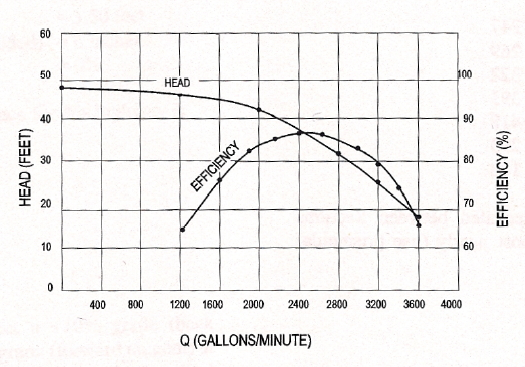
\includegraphics[width=6in]{PumpCurve.png}
   \caption{Lift station performance curve}
   \label{fig:PumpCurve} 
\end{figure}
\clearpage

Determine:
\begin{enumerate}
\item Sketch the system described in the problem statement.
\item Inlet and outlet minor loss coefficients, cite your source of minor loss coefficients.
\item The roughness height for use in head loss calculations, cite your source of roughness height.
\item The energy equation for the system (system curve).
\item The system loss for a discharge of 1200, 1600, 2000, 2400, and 2800 gallons-per-minute. 
    \begin{itemize}
    \item Show the calculation of Reynolds number for the different flow rates. 
    \item Show the determination of the friction factors.
    \end{itemize}
\item The operating discharge for the system using the supplied pump curve.
\item The electric power supplied to the pump to lift the water at the operating point.
\end{enumerate}
\clearpage

\item Water is to be pumped at a rate of 70 liters per second in a 1-kilometer meter long, 200 millimeter diameter pipeline between two reservoirs with an elevation difference of 26 meters. A schematic of the system is shown on Figure \ref{fig:Q2ReservoirWithPump}. The kinematic viscosity of water in the system is $\nu = 1 \times 10^{6} m^2/s$ The
roughness height of the steel pipe is $\epsilon = 0.045 mm$.
\begin{figure}[h!] %  figure placement: here, top, bottom, or page
\centering
   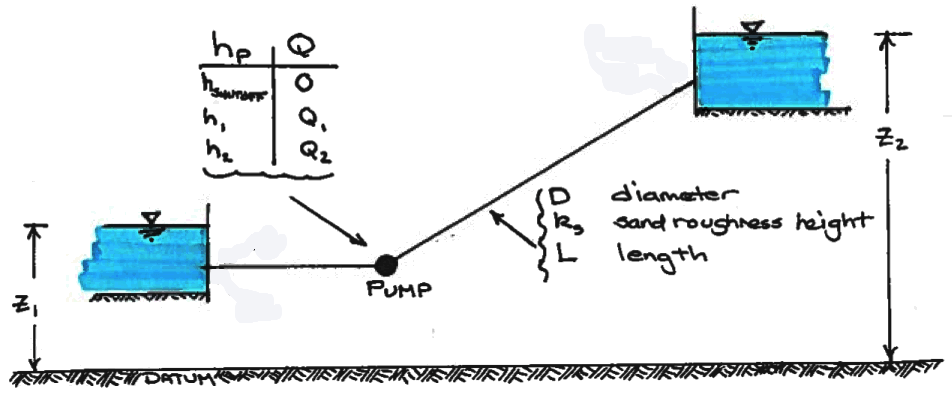
\includegraphics[width=6in]{Q2ReservoirWithPump.png}
   \caption{Pipeline and pump schematic}
   \label{fig:Q2ReservoirWithPump} 
\end{figure}

Determine:
\begin{enumerate}
\item A pump type (from the four curves below) that can supply the required head at the required flow rate.
\item Write the impeller speed for the pump in your selection.
\item Indicate (label on the appropriate pump curve) the operating point of the pump you selected.
\item Estimate the required NPSH for the pump you choose.
\item Demonstrate that $NPSH_a > NPSH_r$ for your pump choice.
\end{enumerate}


\begin{figure}[h!] %  figure placement: here, top, bottom, or page
\centering
   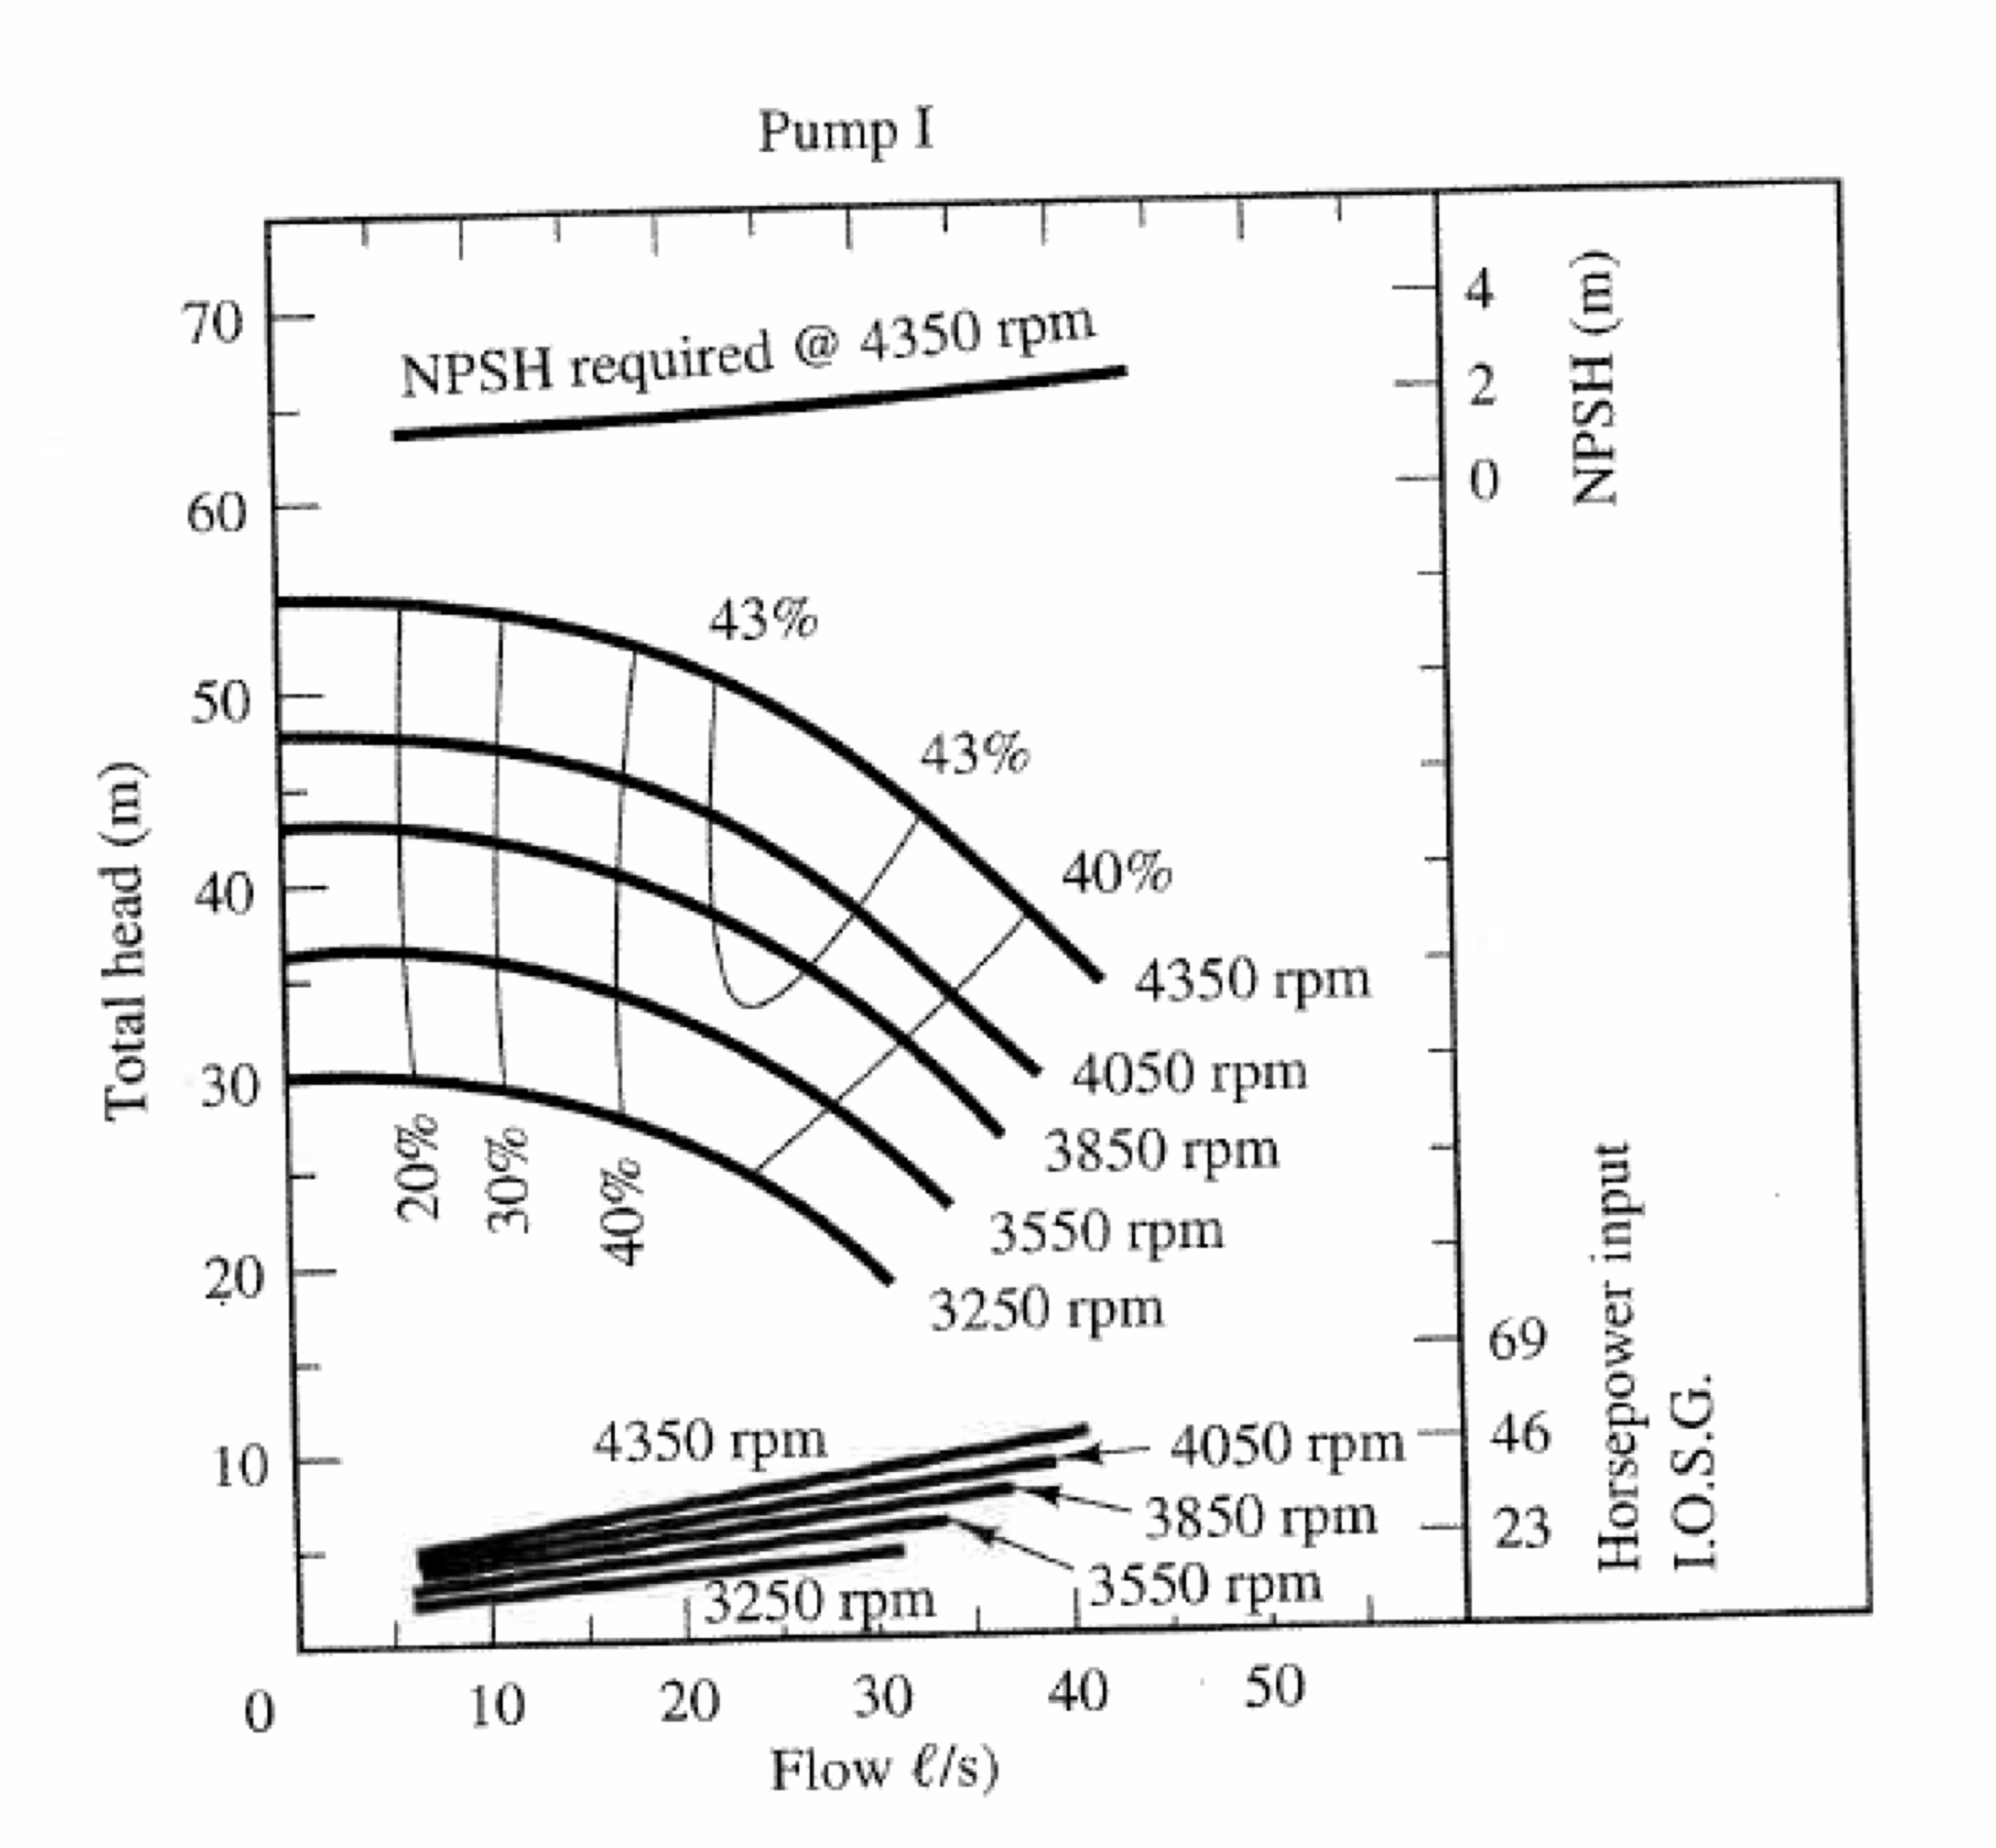
\includegraphics[width=6in]{pump1.png}
   \caption{Pump Type I}
   \label{fig:Pump1} 
\end{figure}

\begin{figure}[h!] %  figure placement: here, top, bottom, or page
\centering
   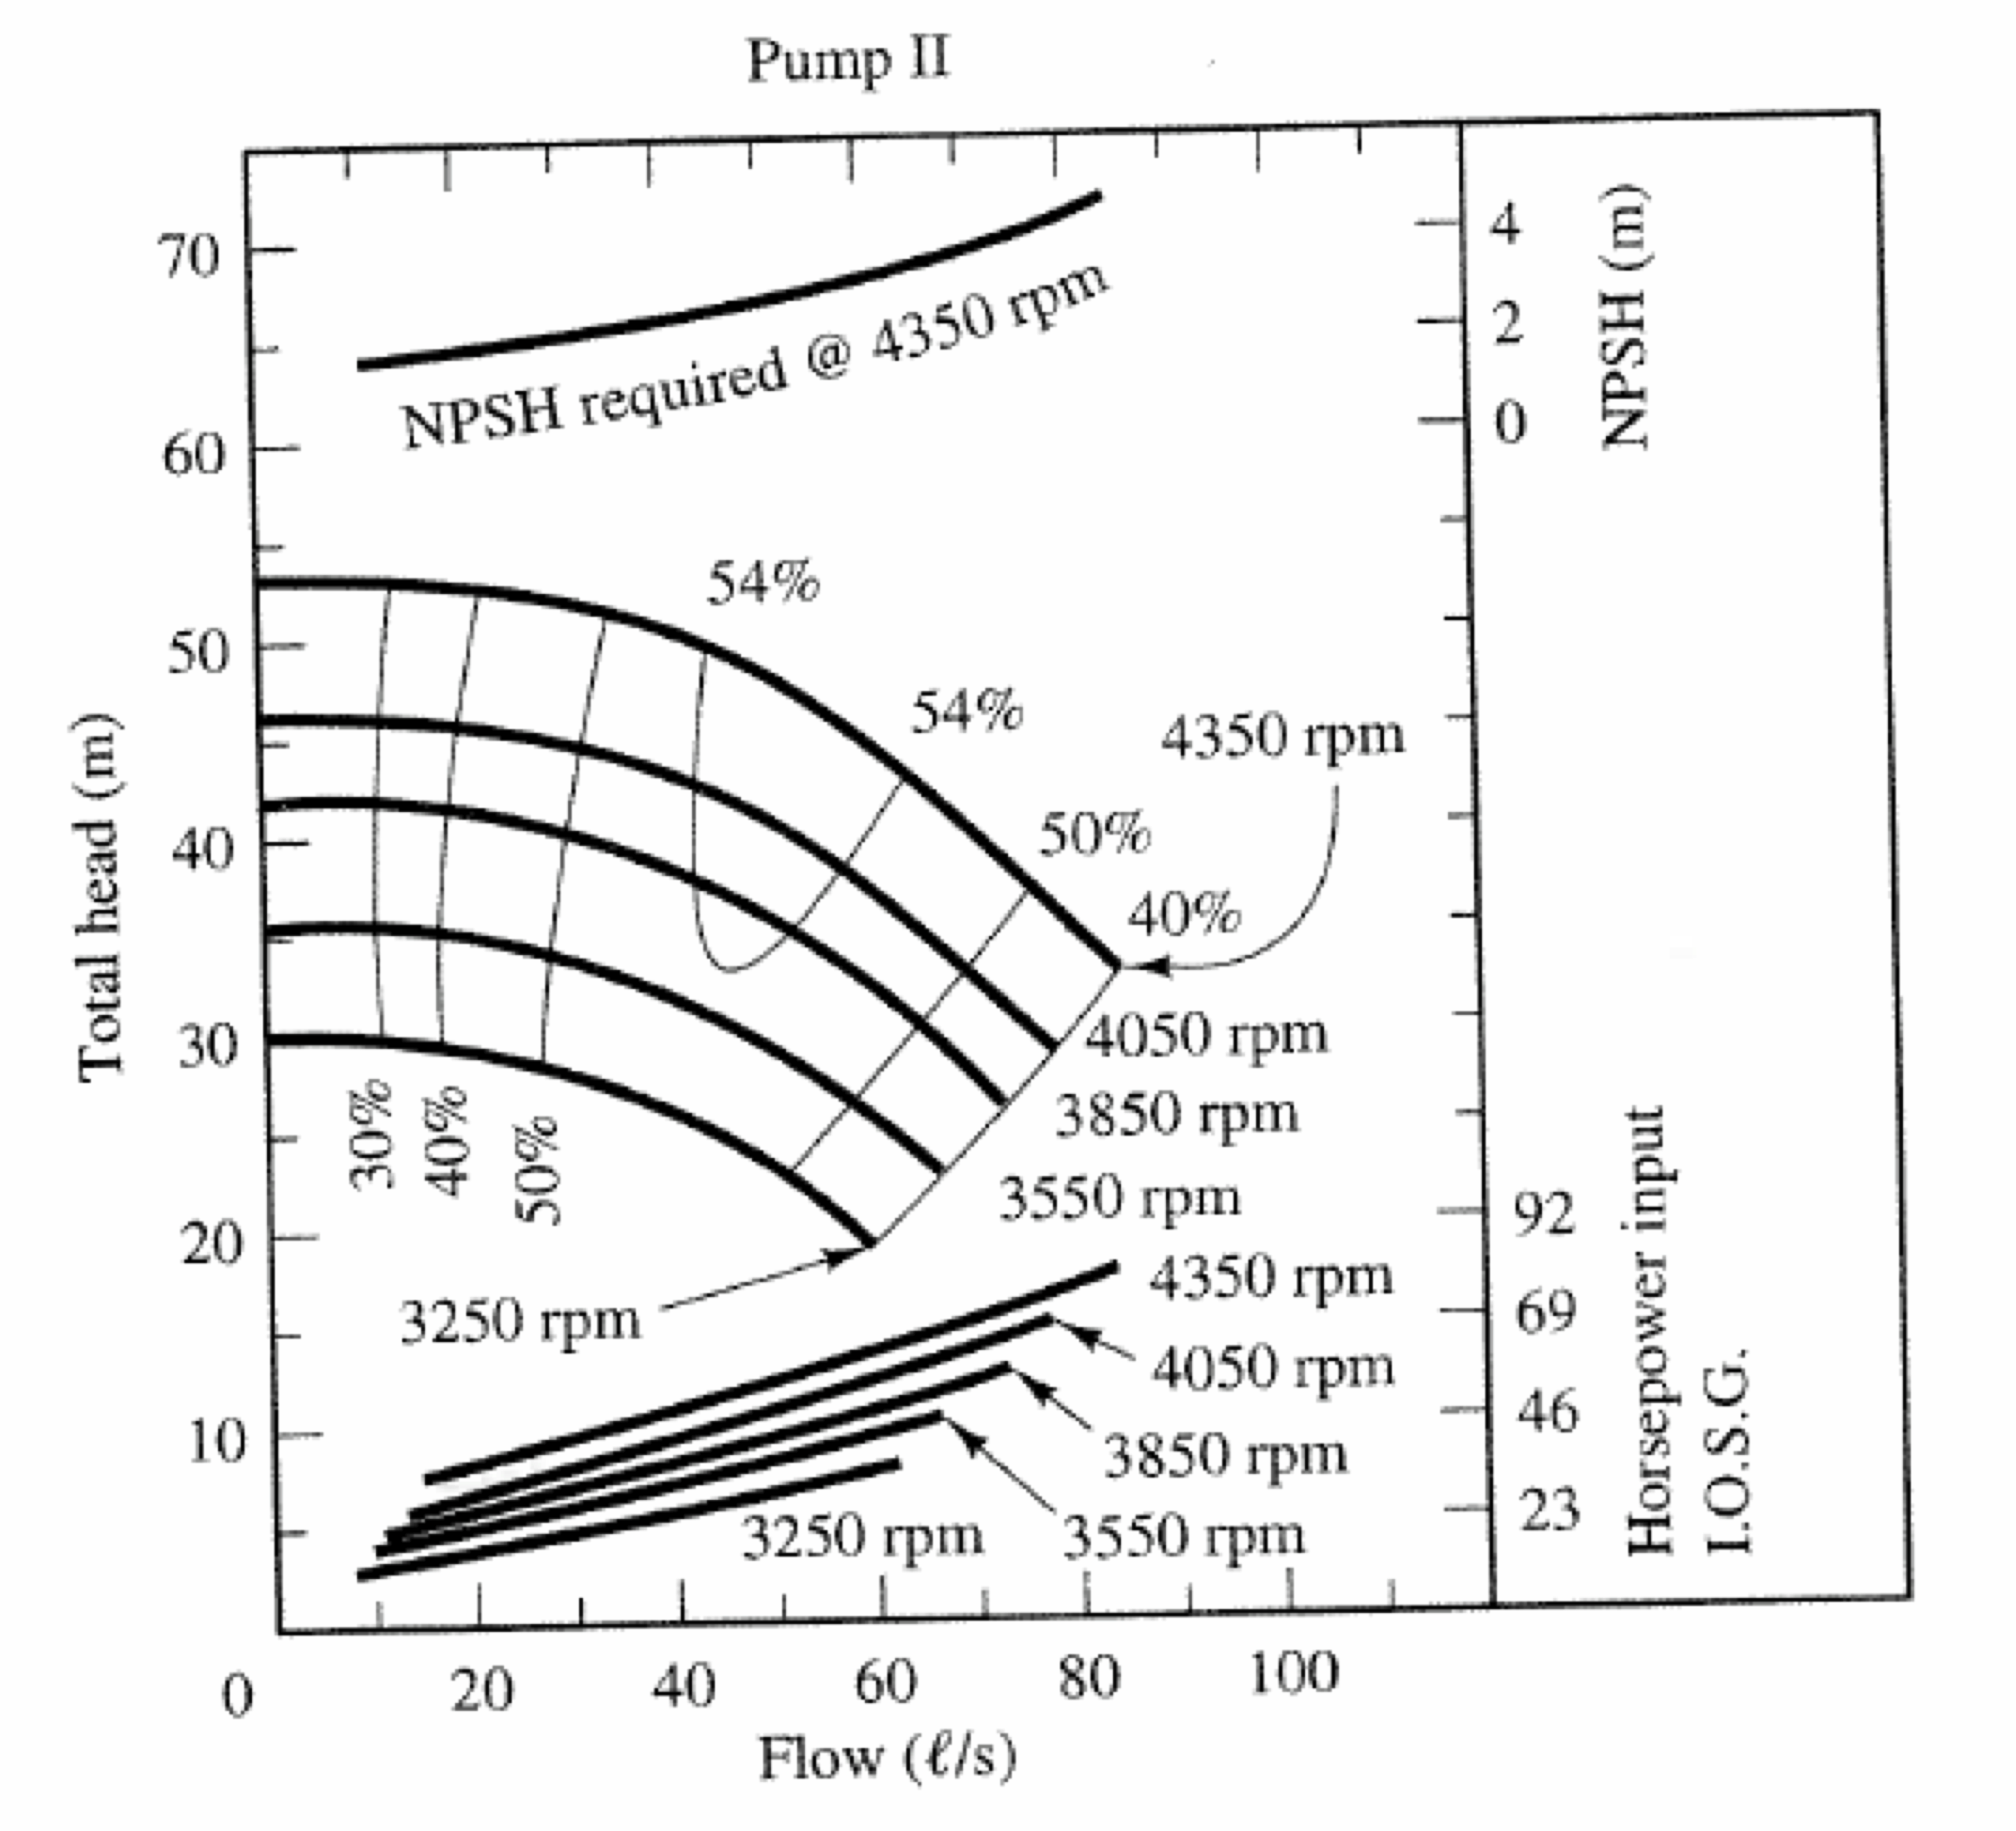
\includegraphics[width=6in]{pump2.png}
   \caption{Pump Type II}
   \label{fig:Pump2} 
\end{figure}

\begin{figure}[h!] %  figure placement: here, top, bottom, or page
\centering
   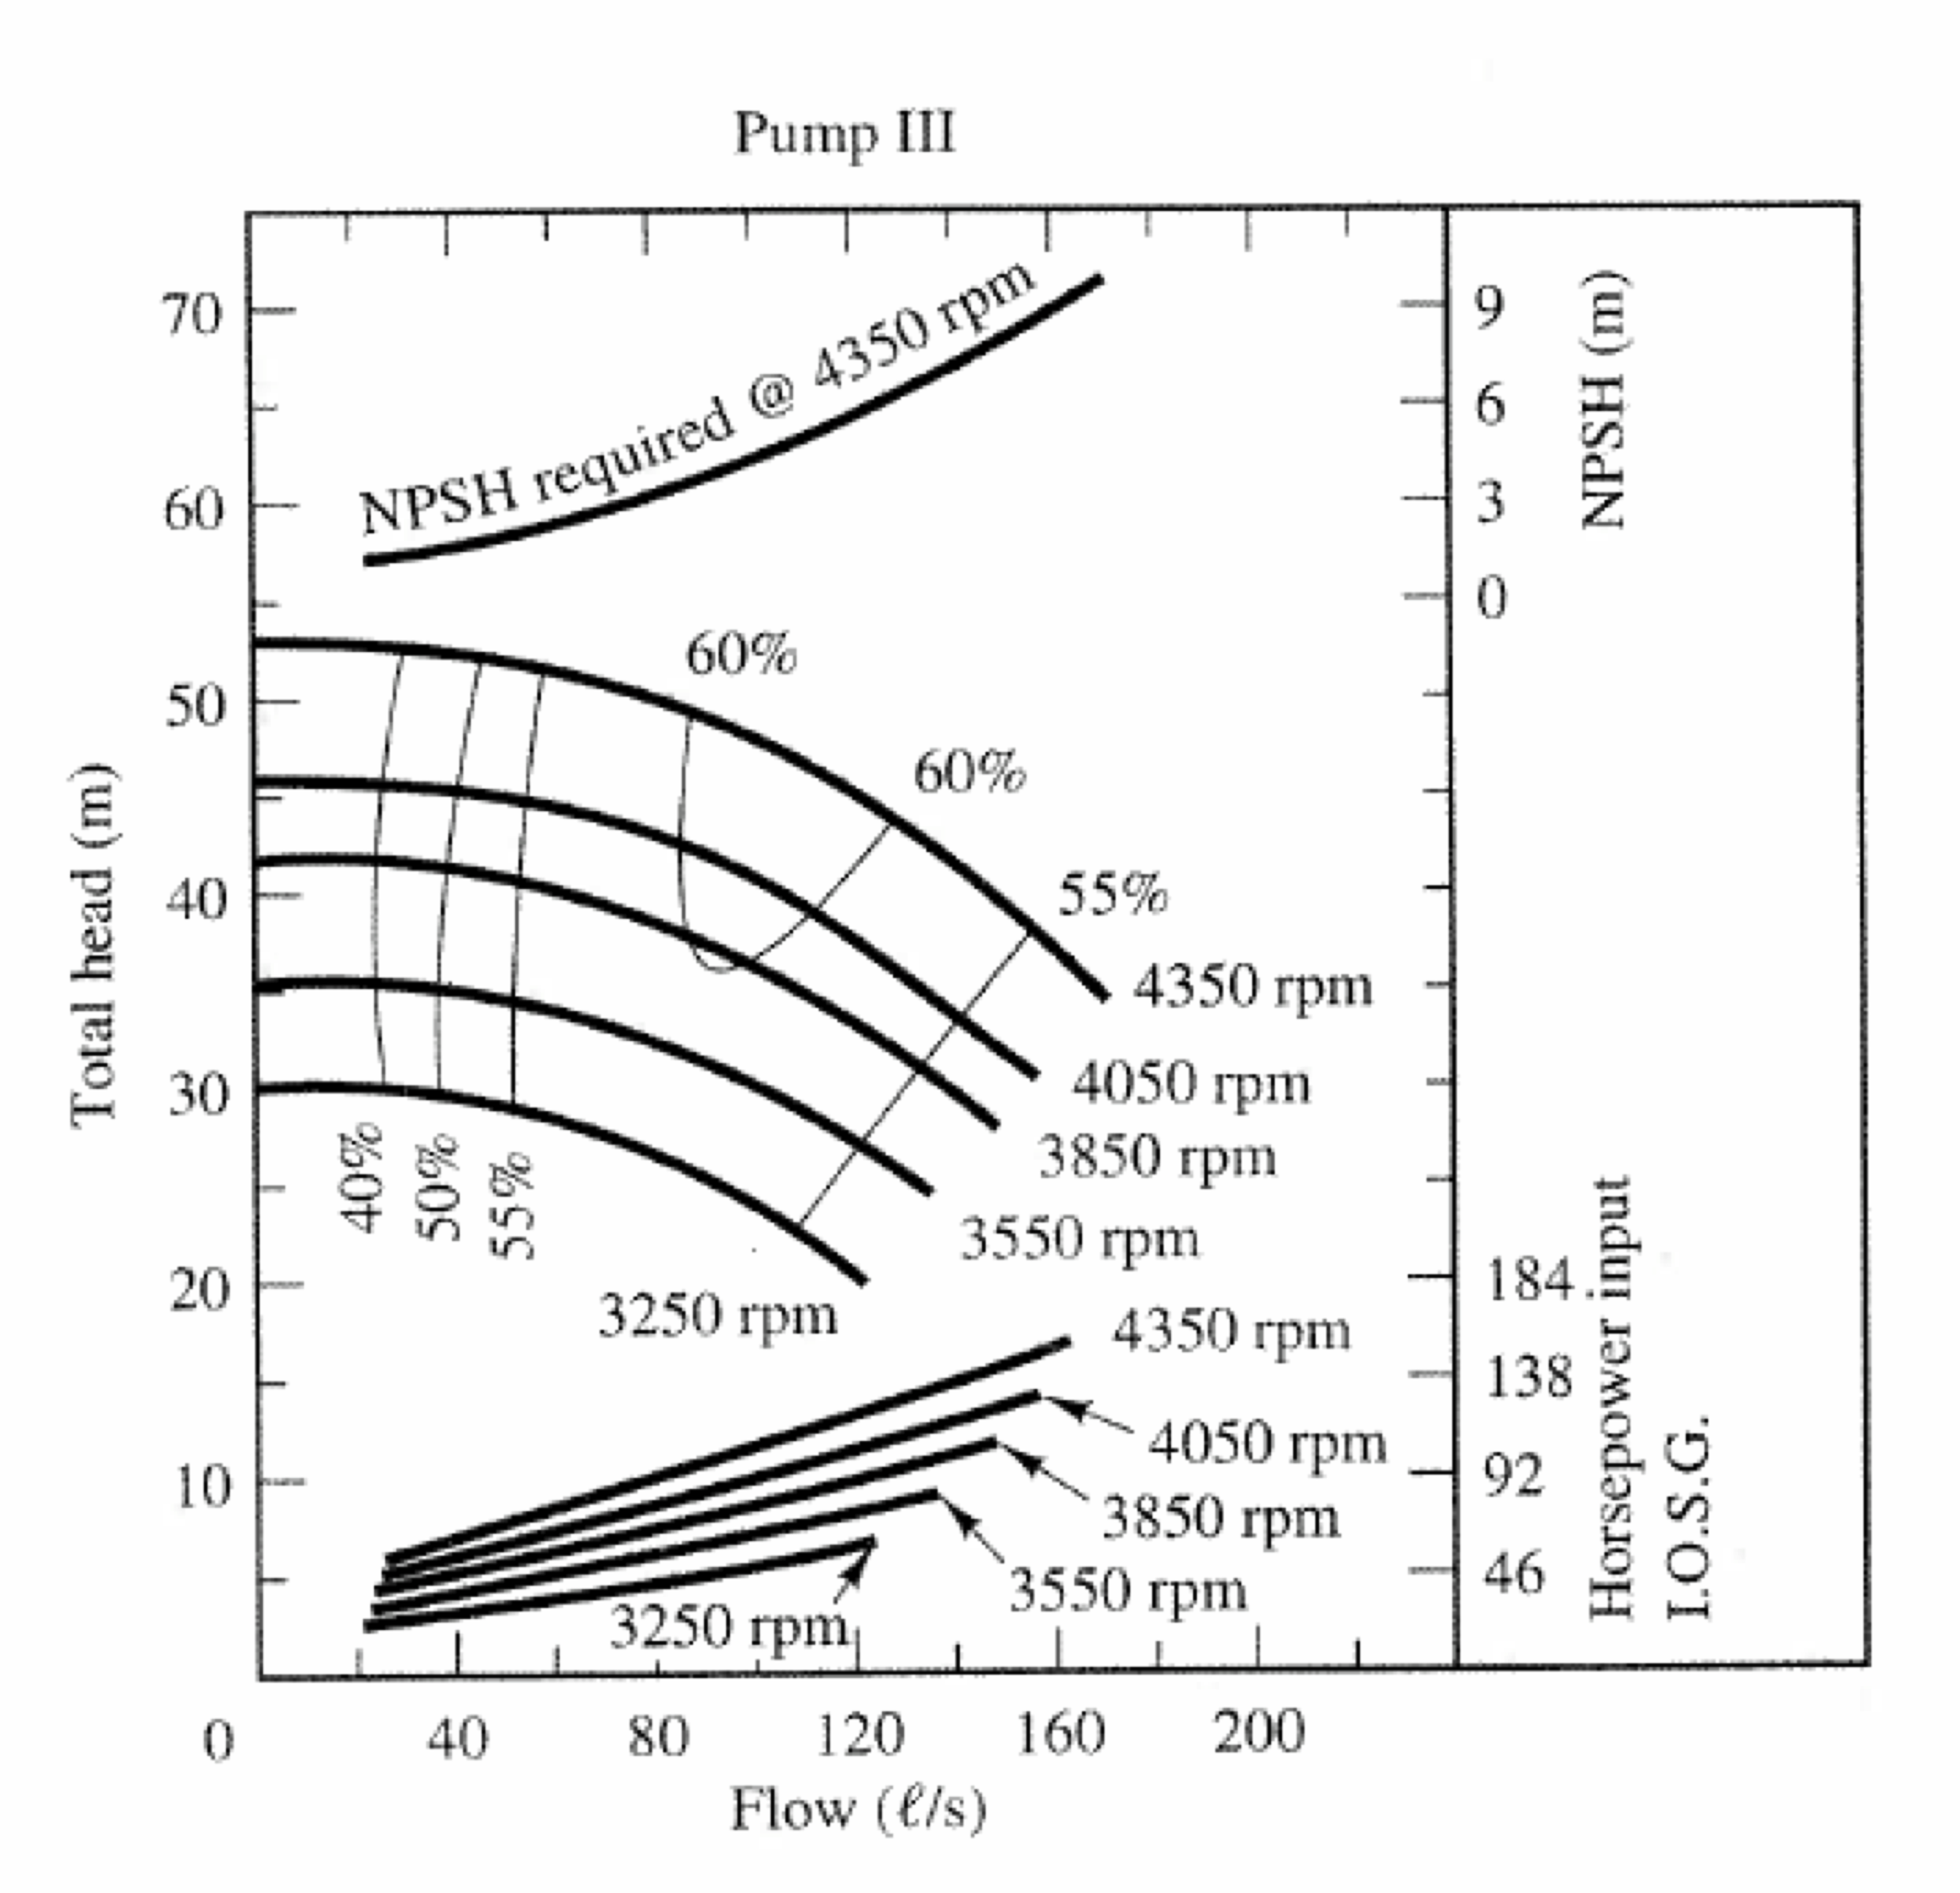
\includegraphics[width=6in]{pump3.png}
   \caption{Pump Type III}
   \label{fig:Pump3} 
\end{figure}

\begin{figure}[h!] %  figure placement: here, top, bottom, or page
\centering
   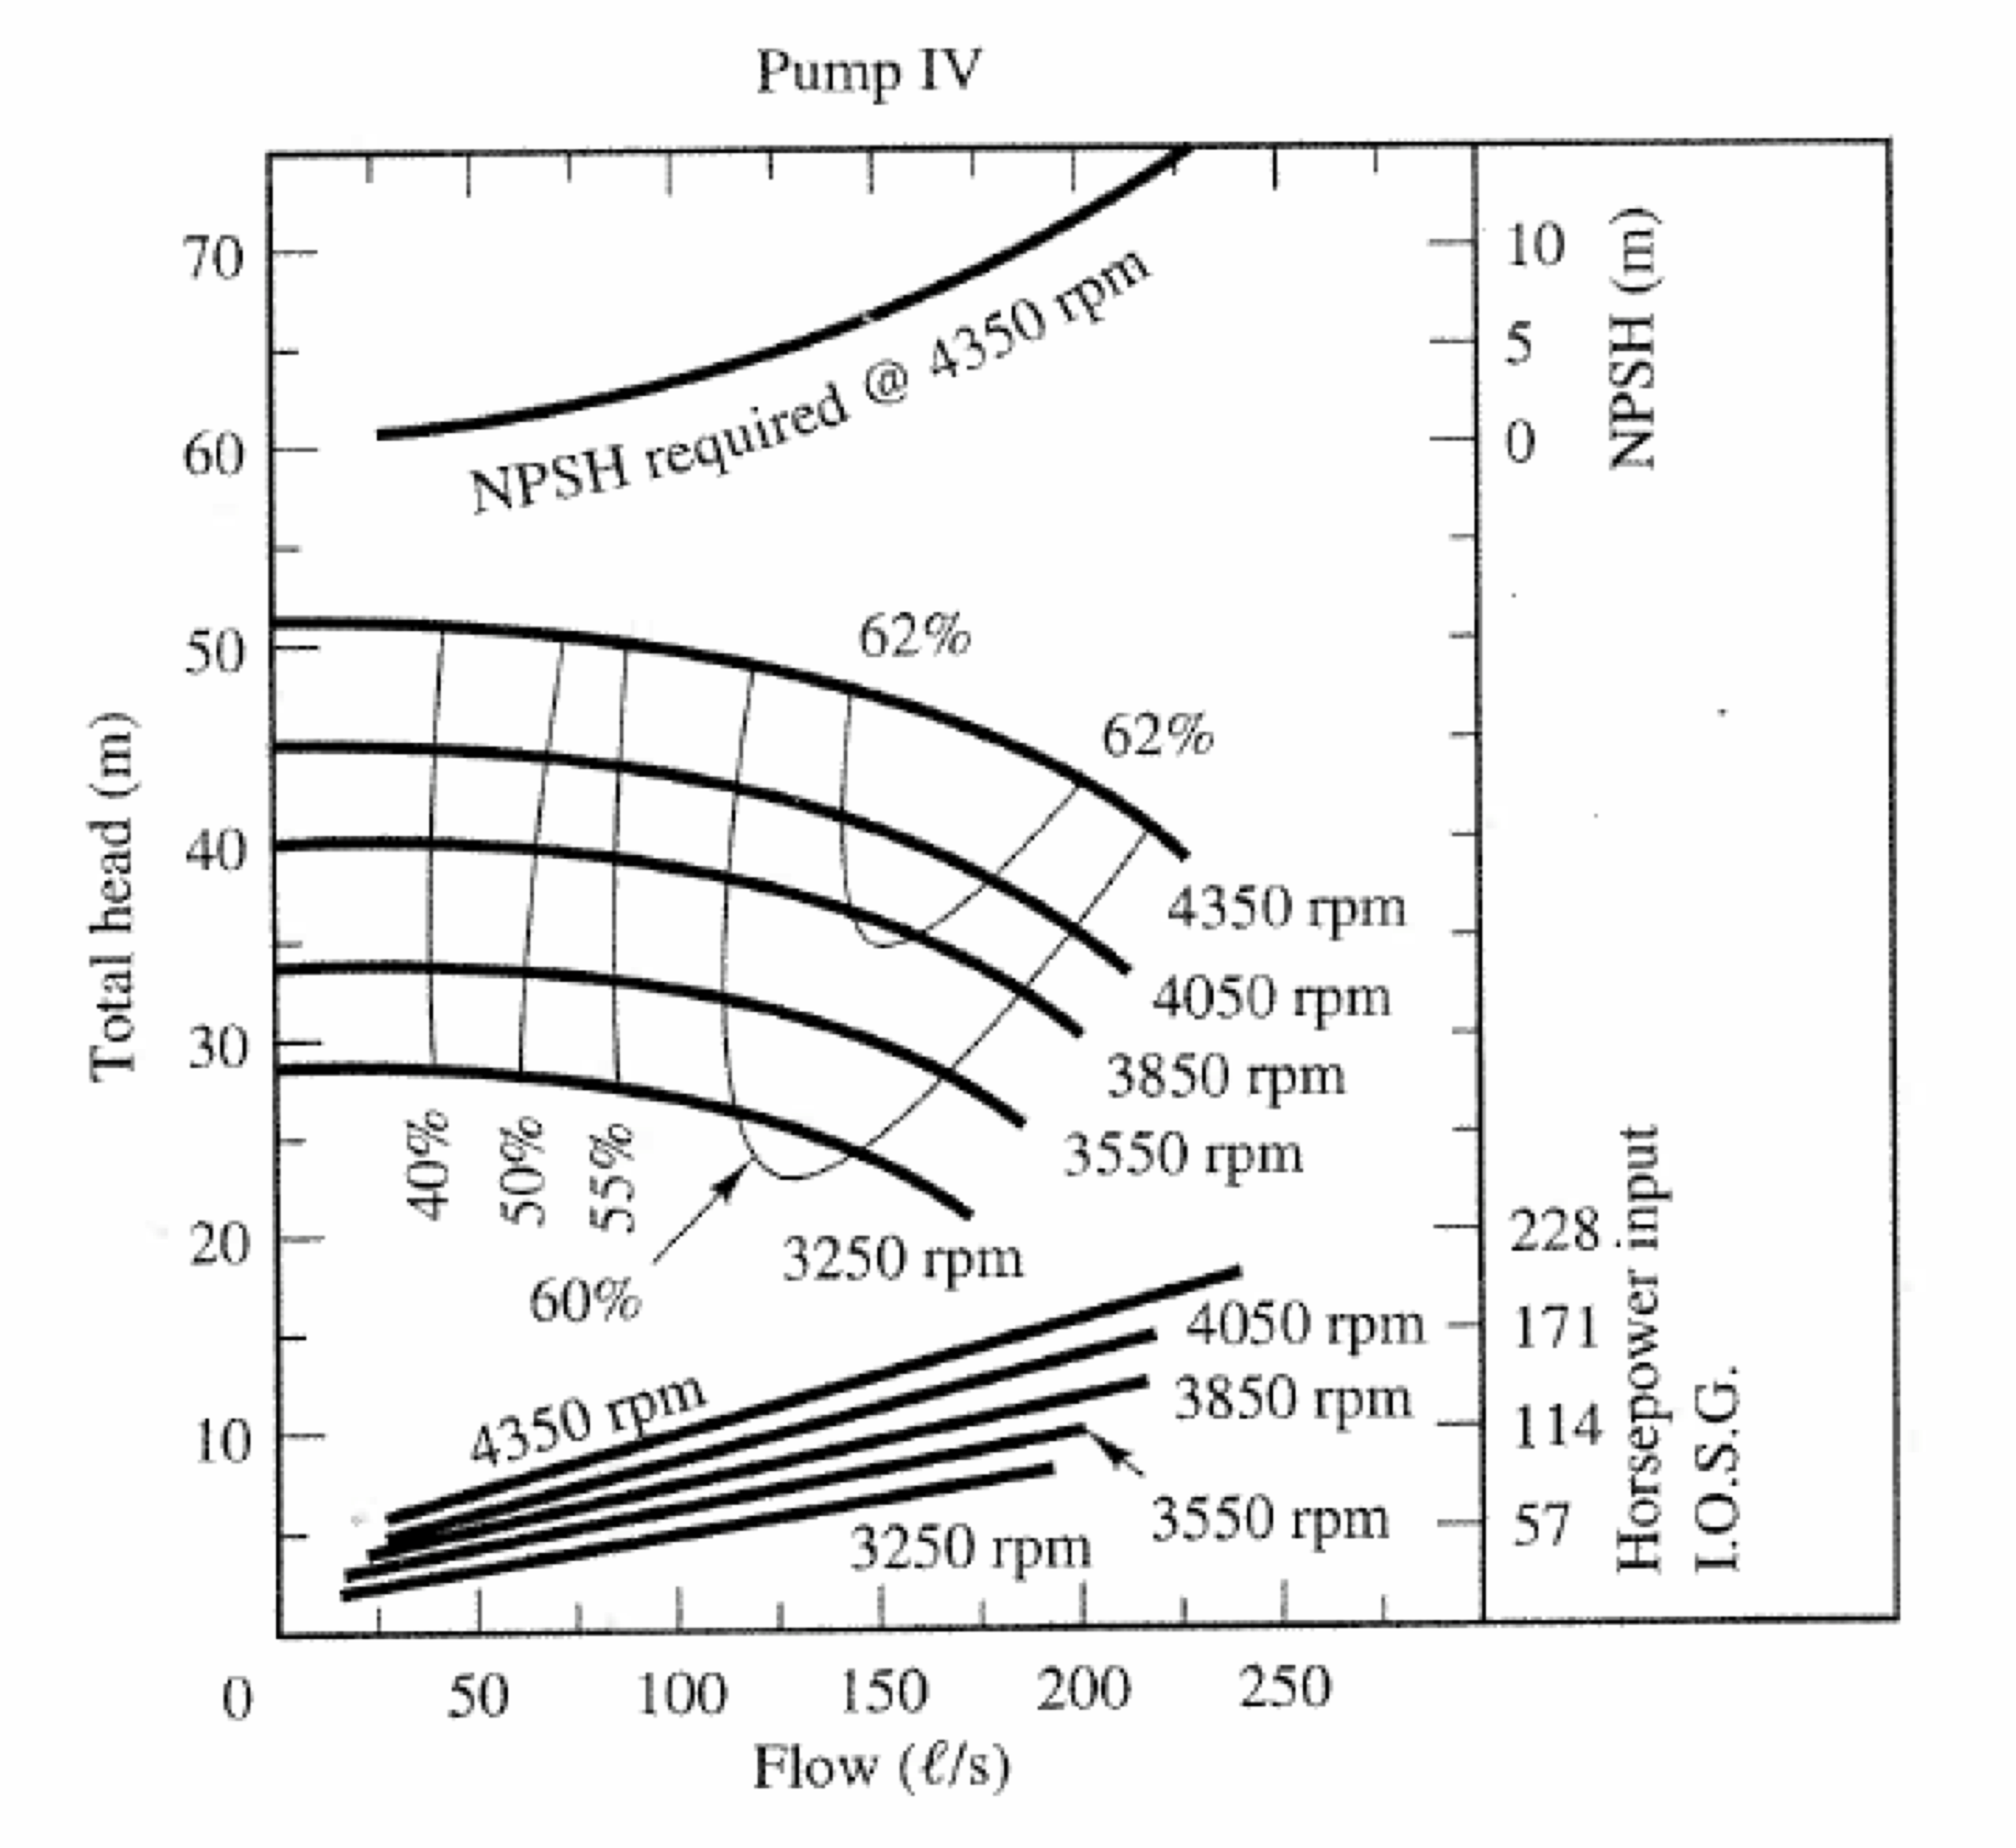
\includegraphics[width=6in]{pump4.png}
   \caption{Pump Type IV}
   \label{fig:Pump4} 
\end{figure}

\end{enumerate}
\end{document}  


% Requires the booktabs if the memoir class is not being used
\begin{table}[htbp]
   \centering
   \caption{Node and Pipe Data}
    \begin{tabular}{p{1in} p{1in} p{1in} p{1in} } % Column formatting, @{} suppresses leading/trailing space
    \hline
    \hline
Pipe ID & Diameter (inches) & Length (feet) & Material \\
\hline
P1 & 8 & 800 & PVC  \\
P2 & 8 & 700 & PVC  \\
P3 & 8 & 700 & PVC  \\
P4 & 8 & 800 & PVC  \\
P5 & 6 & 600 & PVC  \\
\hline
\hline
Node ID & Demand (CFS) & Elevation (feet) & ~~ \\
\hline
N1 & 2.0 & 0.0 & ~~ \\
N2 & 4.0 & 0.0 & ~~ \\
N3 & 3.0 & 0.0 & ~~ \\
N4 & 1.0 & 0.0 & ~~ \\
   \end{tabular}
   \label{tab:PipeData}
\end{table}

Build an EPANET model, using the Hazen-Williams head loss model of the network.
From your preparation, or the completed model:
\begin{enumerate}[a)]
\item Write the node equations of continuity for Nodes 1-4.   
\item Write the head loss equations for each of the pipes in the system.
\item  Make a screen capture of the EPANET program showing your network map, with the Node ID and Node Pressures displayed on the map, and with the Pipe ID and Pipe Flow Rates on the map.
\item Make a table that lists each node name, node elevation, and the resultant pressure in U.S. Customary units.
\item Make a table that lists each pipe name, length, diameter, Hazen-Williams coefficient, and the resultant flow rate in U.S. Customary units.  
\item Determine the flow rate in each pipe of the network, for the case where the total head at Node 1 is 100 feet.
\item Determine the Darcy-Weisbach friction factor in each pipe of the network.
\item Using the results of your flow distribution, determine the head loss from Node 1 to Node 4.
\item Determine the head at Node 4
\item Identify the node with the lowest pressure in your solution.
%\item Compare the head loss from Nodes 1 to 4 determined by EPANET and the by-hand solution in the prior problem.
\end{enumerate}

%Submit the above items as content in a technical memorandum that includes a description of how the model was built and a discussion and interpretation of the results.

Attach the EPANET output report to your solution.
\clearpage
%%%%%%%%%%%%%%%%%%%%%%%%%%%%%%%%%%%%%%%%%%%%%%%%%%%%%%%
%%%%%%%%%%%%%%% PROBLEM 2 %%%%%%%%%%%%%%%%%%%%%%%%%%%%

\item Figure \ref{fig:primary-network} is a layout of a water distribution system for the SomewhereUSA subdivision. 
The blue line segments are pipes (ductile iron) and are labeled (P1, P2, . . . ). The blue circles are nodes and are labeled (N1, N2, . . . ).  The yellow polygons represent the demand lots assigned to each node. For example, node N2 supplies the six (6) individual lots located near the node.

\begin{figure}[h!] %  figure placement: here, top, bottom, or page
   \centering
   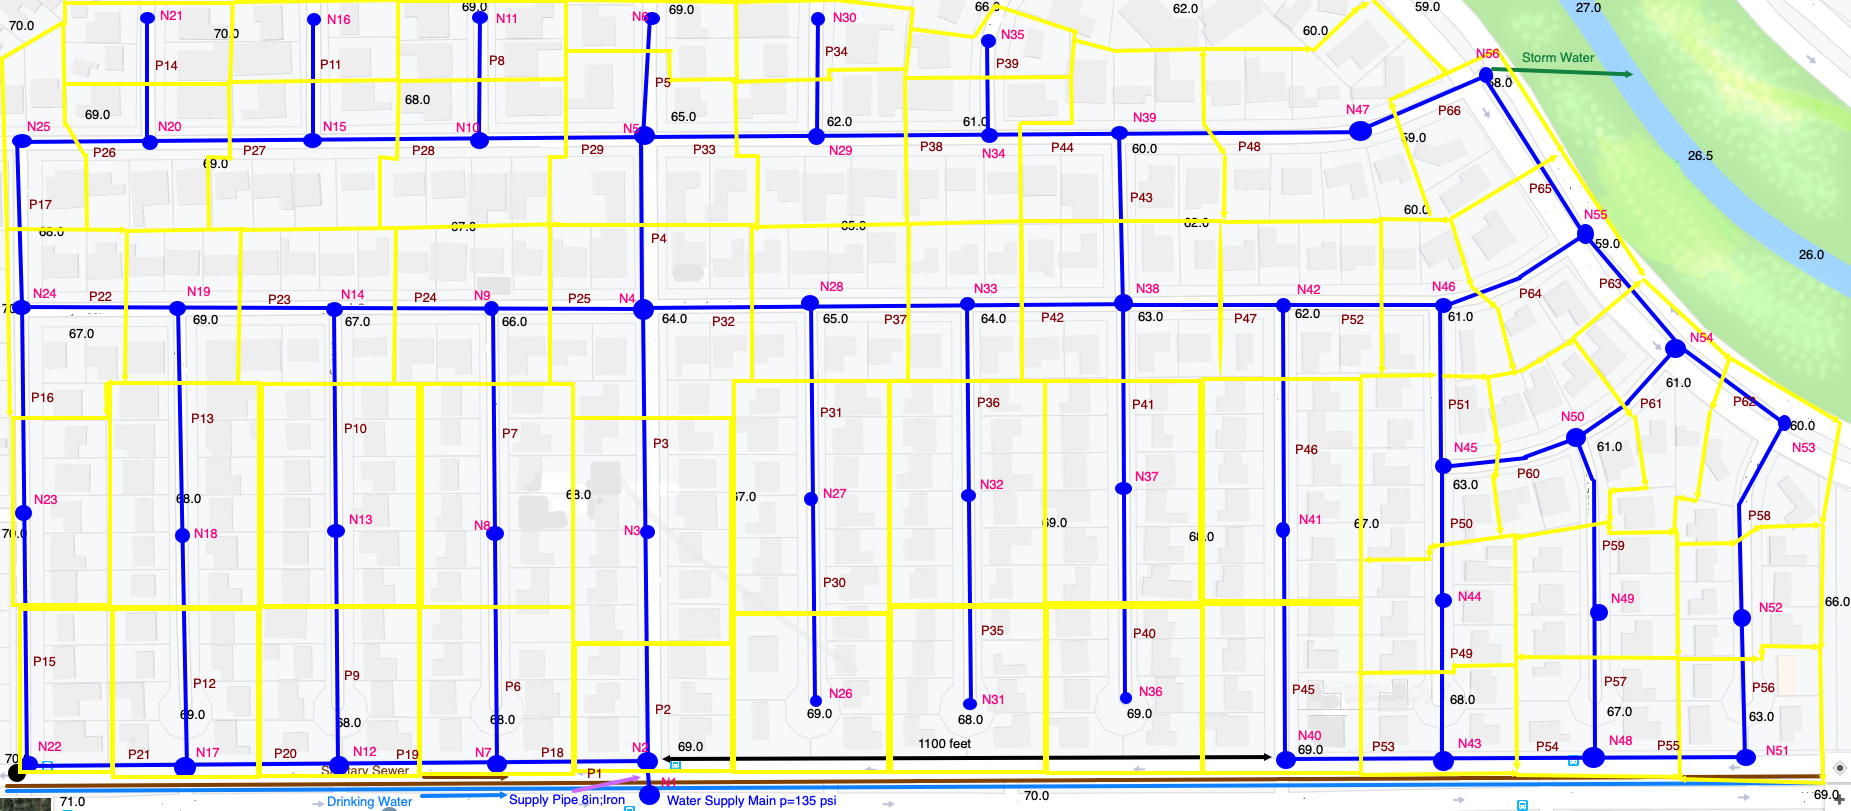
\includegraphics[width=6.5in]{SomewhereClipNodes.png} 
   \caption{Somewhere USA Water Distribution (Skeleton) System}
   \label{fig:primary-network}
\end{figure}

The distribution system is connected to the supply main at node N1. 
This large water main supplies water at 135 psi. pressure. 
The pipe connecting node N1 to N2 is an 8-inch diameter, ductile iron pipe. The remaining pipes are 2-inch diameter, ductile iron pipe.

The system is to be modeled using the United States Environmental Protection Agency, EPANET  hydraulic and water quality simulator. Use RG-195 and the San Marcos Texas manual for statutory requirements as necessary:

\begin{enumerate}[1)]
\item Using the naming convention in the drawings, determine the individual pipe lengths and produce a table of pipe length, and diameter by pipe ID. Include this table in your solution report;
\item Produce a land surface elevation map; include the map in your solution report (you did this in an earlier exercise, you can reuse your map and need not create a new one;
\item Using the naming convention in the drawings, determine the individual node elevations (offset as necessary to ensure the pipe network is buried a sufficient depth throughout the subdivision) and produce a table of node elevation by node ID;
\item Determine magnitude and location of minimum pressure in the system at average demand (reuse your earlier exercise solutions);
\item Determine magnitude and location of minimum pressure in the system at peak demand;
\item Determine magnitude and location of maximum pressure in the system at average demand;
\item Determine magnitude and location of maximum pressure in the system at peak demand;
\item Determine if there are low-pressure portions of the system that need to be mitigated by changing pipe diameters, if so, adjust the diameters and present the adjusted design as a second, independent simulation;
\item Apply a demand pattern multiplier and simulate time-varying behavior in the distribution system;
\end{enumerate}

\end{enumerate}

%\begin{thebibliography}{}
%
%\bibitem[\protect\citeauthoryear{Swamee and Jain}{Swamee and Jain}{1976}]{jain1976}
%Swamee and Jain, A. K., 1976. Explicit equations for pipe-flow problems.  ASCE J. of Hyd. Div., 102(HY5) pp. 657-664 
%
%
%\end{thebibliography}